\documentclass[a4paper]{article}
\usepackage[utf8]{inputenc}
\usepackage[natbib,sorting=none]{biblatex}
\usepackage{graphicx}
\usepackage{acronym}
\usepackage{indentfirst}
\usepackage{requirements} %custom package
\usepackage[htt]{hyphenat} %stops word separation on new line
\usepackage{fancyhdr}
\usepackage{enumitem}
\usepackage{listings}
\usepackage{xcolor}

\definecolor{commentgreen}{RGB}{2,112,10}
\definecolor{eminence}{RGB}{108,48,130}
\definecolor{weborange}{RGB}{255,165,0}
\definecolor{frenchplum}{RGB}{129,20,83}

\addbibresource{references.bib}

\begin{document}
\setlist[enumerate]{label=\alph*),leftmargin=0.4cm, topsep=0cm}
\setlength{}{}
\pagenumbering{none}
\begin{figure}[!h]
	\centering
	
\includegraphics[width=80mm]{images/poli-logo.png}
\end{figure}
\hfill
\begin{center}
    \fontsize{18px}{6mm}\selectfont \textsc{\textbf{Software Engineering II project}}
\end{center}
\begin{center}
    \fontsize{12px}{4mm}\selectfont \textsc{Academic Year: 2018/2019}
\end{center}
\hfill
\hfill
\begin{figure}[!h]
	\centering
	
\includegraphics[width=120mm]{images/trackme-logo.png}
\end{figure}
\hfill
\hfill
\begin{center}
    \fontsize{22px}{8mm}\selectfont \textsc{\textbf{Requirement Analysis and\\ Specification Document}}
\end{center}
\begin{center}
    \fontsize{14px}{4mm}\selectfont \textsc{{Draft Version 0.1 - 11/10/2018}}
\end{center}
\hfill
\hfill
\begin{center}
\fontsize{14px}{4mm}\selectfont \textsc{\textit{Davide Rutigliano -  903616}}
\end{center}

\begin{center}
\fontsize{14px}{4mm}\selectfont \textsc{\textit{Claudio Ferrante - 903417\\}}
\end{center}

\begin{center}
\fontsize{14px}{4mm}\selectfont \textsc{\textit{Davide Matta - 903616}}
\end{center}
\pagenumbering{roman}
\tableofcontents
\newpage
\addcontentsline{toc}{subsection}{Use Cases Summary}
\renewcommand\listtablename{Use Cases Summary}
\listoftables
\newpage
\addcontentsline{toc}{subsection}{UML Diagrams List}
\renewcommand\listfigurename{UML Diagrams List}
\listoffigures
\newpage
\rfoot{
\includegraphics[width=30mm]{images/trackme-logo-mini.png}}
%%%%%%%%%%%%%%%%%%%%%%%%%%%%%%%%%%%%%%%%%%%%%%%%%%%%%%%%%%%%%%
\newpage
\pagestyle{fancy}
\pagenumbering{arabic}
\section{Introduction}

    \subsection{Purpose}
    This Requirement Analysis and Specification Document addresses the description in terms of functional and non-functional requirements of \textit{TrackMe}, a new health monitoring application.
    
    This specification is aimed at giving an explanation both of the problem and of the proposed software-based solution by pointing out different features of the application; in addition, is intended to model and describe the system itself, its requirements, its constraints, its components and how it interacts with the world and the users. Moreover, this specifications also addresses some relevant QoS characteristics that the system should guarantee.
    
    The analysis is focused on requirements elicitation and use cases description through well known standards for specification documents such as \textit{UML} for Use Case, Sequence and Activity Diagrams \cite{rumbaugh2004unified} and \textit{Alloy} for formal analysis \cite{jackson2006software}.
        
    This document is directed and highly recommended to software designers and developers interested in the deployment of the proposed system.
    
    \subsection{Scope and Audience}
        \subsubsection{Description of the given problem}
        \textit{TrackMe} is a company that wants to develop an ease of use health monitoring application which offers different services for both young and old people who needs to keep track of their personal data in order to to keep their health safe.
        
        The system should provide an efficient data acquisition facility which gives the possibility to verified \textit{third-party} signed onto the service to request health status information about subscribed customers. The application may also allow \textit{individual} users to connect \textit{external devices} such as smart-watches or similar, to perform a more detailed data acquisition and monitoring.
        
        In addition, the \textit{third-party} may also provide a personalized and non intrusive SOS service for elderly people that may also request for it.
    
        Moreover, through the \textit{Track4Run} service, \textit{TrackMe} wants to provide to third-parties signed in the application to create a new run, a competition in which other users can either participate as \textit{athletes} or watch as \textit{spectators}. Additionally, this feature may exploits other service functionality for keeping track of athletes progresses and for helping them to prevent major accident happen during the run.
                
        \subsubsection{Description of the proposed system}
        The proposed solution consists of a back-end server application that manages users' registration, login and data and allows to keep everything synchronized between the two front-end applications:
        \begin{itemize}
            \item a web-based application to supply to the end user an ease of use interface web interface for \textit{TrackMe};
            \item a mobile application that allows the user to easily access the system from the smartphone.
        \end{itemize}
        
        The application will provide both \textit{"Sign-on"} and \textit{"Sign-in"} pages and will be able to register new users and to check credentials used to login.
        
        To register himself an user must provide an username and a password as well as his/her personal information. To be logged in, the user should send through the login form his credentials which the system will use to authenticate him/her.
        
        \textit{TrackMe} may further yield an interface that allows individual users to connect external devices and a method for acquiring data from it.
        
        The application should also provide to third-parties two possible data request options:
        \begin{itemize}
            \item individual data request: sent directly to the individual if they know an  individual by his/her social security number or fiscal code in Italy;
            \item group data request: access  to  anonymous  data  of  groups  of  individuals, if \textit{TrackMe}  that  approves  them  if  it  is  able  to  properly  anonymize  the  requested  data.
        \end{itemize}
        
        Moreover, the system implements \textit{Data4Help} services to manage individual's personal data and provide them to third-parties who requested for. In addition, there should be an interface both for third-party and individual users registered to \textit{Data4Help} that wants to enable an \textit{Automated-SOS} service. This feature should be able to use users' data to monitor their health status and, when such parameters are below certain thresholds, sends the location of the customer to an ambulance.
        
        Furthermore, the software should provide to users that wants to use \textit{Track4Run} all the facilities they need such as a page for the creation of a new run with all the information (track, date and time) and two different pages to allow both spectators and athletes to watch or enroll to existing run.
        
        \subsubsection{Goals}
        
        \begin{description}
            \item[G.01] Let the user register on the system
            \item[G.02] Let the user login/logout from the application
            \item[G.03] Let the individual user connect an external device
            \item[G.04] Let the third-party make requests to a specific individual
            \item[G.05] Let the third-party make requests to groups of individuals
            \item[G.06] Let the third-party subscribe to individuals' data
            \item[G.07] Let the user manage his profile
            \item[G.08] Let the individual accept/refuse third-party requests
            \item[G.09] Let the third-party enable automated-Sos service
            \item[G.10] Let the individual enable automated-Sos choosing among third-party that has enabled the service
            \item[G.10] Let the organizer create a new run
            \item[G.11] Let the organizer delete a run
            \item[G.12] Let the organizer start a new run
            \item[G.13] Let the athlete enroll to a run
            \item[G.14] Let the athlete unroll to a run
            \item[G.15] Let the spectator watch a run
        \end{description}
    
    \subsection{Document Overview}
        This initial part of the document is intended to provide both an overview of the problem and an idea of the proposed solution.
        
        Following section is aimed at giving a more detailed description of the proposed system, by meaning of the application point of view. Additionally, it addresses user characteristics, dependencies and constraints.
        
        Third chapter shows a detailed analysis of \textit{TrackMe} in terms both functional and non-functional requirements of the system. Furthermore, takes into account definition of all use cases, their description through UML diagrams and their mapping on requirements.
        
        Endmost section illustrates \textit{Alloy} models including purpose, proof and explanation. In addition, describes worlds obtained by running them.
        
        Further, there is a list of tables and a list of figures representing respectively use cases and diagrams in order to help the reader to understand them and navigate the specification.
        
    \subsection{Definition, Acronyms and  Abbreviations}
            \subsubsection{Keywords}
            The key words “MUST”, “MUST NOT”, “REQUIRED”, “SHALL”, “SHALL NOT”, “SHOULD”, “SHOULD NOT”, “RECOMMENDED”, “MAY”, and “OPTIONAL” in this document are to be interpreted as described in RFC 2119 \cite{bradner1997key}.
            \subsubsection{Definition of Terms}
            This document uses several terms that might be more loosely used elsewhere. These terms are defined here as they will be used later on in this document.
                \begin{description}
                    \item[\textbf{User}] a general definition of a customer registered into the application
                    
                    \item[\textbf{Individual}] a single person \textit{User}, identified either by SSN or by FC number
                    \item[\textbf{Third-Party}] an organization \textit{User}, identified by VAT number
                    
                    \item[\textbf{Subscribed User}] an individual for which one or more third party have done a request accepted by the individual itself
                    
                    \item[\textbf{External Device}] an external device such as a smart-watch or similar devices
                    
                    \item[\textbf{Run}] a competition organized and managed by an \textit{Organizer} to which \textit{Athletes} and \textit{Spectators} can enroll as participant or watchers
                    
                    \item[\textbf{Organizer}] either an \textit{Individual} or a \textit{Third-Party} that uses \textit{Track4Run} service to create a new \textit{Run}
                    
                    \item[\textbf{Athlete}] an \textit{Individual} enrolled to an already existing \textit{Run}
                    
                    \item[\textbf{Spectator}] either an \textit{Individual} or a \textit{Third-Party} that is watching an already existing \textit{Run}
                    
                    \item[\textbf{TrackMe}] the \textit{"system to be"}
                    
                    \item[\textbf{Data4Help}] a data monitoring service provided by \textit{TrackMe}
                    
                    \item[\textbf{Automated-SOS}] an SOS service built on top of \textit{Data4Help}
                    
                    \item[\textbf{Track4Run}] run management service offered by \textit{TrackMe} application
                    
                    \item[\textbf{Credential}] as used in this document, is a combination of both username and password used by an \textit{User} to authenticate him/herself during the Log-in phase
                \end{description}
                
            \subsubsection{Abbreviations}
            \begin{itemize}
                \item $[$An$]$: Assumption number n
                \item $[$Cn$]$: Constraint number n
                \item $[$Dn$]$: Dependency number n
                \item $[$Gn$]$: Goal number n
            \end{itemize}
            
            \subsubsection{Acronyms}
            \begin{acronym}
                \acro{RASD}{Requirement Analysis and Specification Document}
                \acro{UML}{Unified Modelling Language}
                \acro{QoS}{Quality of Service}
                \acro{SSN}{Social Security Number}
                \acro{FC}{Fiscal Code}
                \acro{VAT}{Value Added Tax}
                \acro{BT}{Bluetooth}
                \acro{NFC}{Near Field Communication}
                \acro{GPS}{Global Positioning System}
            \end{acronym}
            
    \subsection{References}
        \printbibliography[heading=none]
%%%%%%%%%%%%%%%%%%%%%%%%%%%%%%%%%%%%%%%%%%%%%%%%%%%%%%%%%%%%%%
\newpage
\section{Overall Description}
    \subsection{Product Perspective}
    
         TODO:
    Describe the product's context and origin. Is it the next member of a growing product family, the next version of a mature system, a replacement for an existing application, or an entirely new product? If this Software Requirements Specification (SRS) defines a component of a larger system, state how this software relates to the overall system and identify major interfaces between the two.  
    
    
    %%%%%%%%%%%% pretty sure this is the wrong place for this %%%%%%%%%%%%%%
    This section is intended to provide a full description of the proposed system by meaning of \textit{Domains} and \textit{Phenomena} \cite{zave1997four}.
    
    The \textit{Machine Domain} is the set of phenomena that the machine can control: data structures, algorithms, devices and inputs it can get from the world.
    
    In contrast, the \textit{World Domain} is the real-life context in which the \textit{Machine} will be introduced. This is the part of the real-world in which the Machine’s actions will be observed.
    
    The World and the Machine are connected too, because the latter should interact with the first one: this interaction is done through \textit{Shared Domain}, whose phenomena are observable both by the Machine and by the World. Shared Phenomena include events in the real world that the Machine can directly sense and actions in the real world that the Machine can directly cause.
    \begin{table}[!ht]
    \centering
    \begin{tabular}{|l|l|l|l|}
    \hline
     \textbf{Phenomenon} & \textbf{World} & \textbf{Machine} & \textbf{Shared}\\ \hline
     Registration/Login/Manage Profile & & & X \\ \hline
     Application logic & & X & \\ \hline
     Accept/Refuse/Send Request & & & X \\ \hline
     Database Query & & X & \\ \hline
     Connect External Device & & & X \\ \hline
     GPS Tracking & & X & \\ \hline
     Enable Sos & & & X \\ \hline
     Locate nearest Ambulance & & & X \\ \hline
     Accident & X & & \\ \hline
     Create/Delete/Enroll/Watch/Start Run & & & X \\ \hline
     & & & \\ \hline
     NOT FINISHED YET & X & X & X \\ \hline
     & & & \\ \hline
    \end{tabular}
    \end{table}
    
    %%%%%%%%%%%%%%%%%%%%%%%%%%%%%%%%%%%%%%%%%%%%%%%%%%%%%%%%%%%%%%%%%%%%%%
    
    \subsubsection{Class Diagram}
    
    \subsubsection{State Charts}
    
    \subsection{Product Functions}
    \textit{TrackMe} will provide three services: \textit{Data4Help}, \textit{Automated-SOS} and \textit{Track4Run}.
    
    \subsubsection{Data4Help}
    \textit{Data4Help} is the main service: it allows the registration of individuals who by registering consent to provide their personal data to \textit{Track4Me}. Data can be made available to third parties under specific conditions.
    
    \subsubsection{Automated-SOS}
    \textit{Automated-SOS} is built on top of \textit{Data4Help} and provides individuals the ability to subscribe to a third party that has enabled the service. When the individual's health parameters are below a certain threshold an ambulance shall be called to the individual's position under certain time constraints.
    
    \subsubsection{Track4Run}
    \textit{Track4Run} is also built on top of \textit{Data4Help} and allows third parties to create new runs where athletes can participate. Athletes' position can be tracked and it will be sent to all spectators that are watching the run.
    
    \subsection{User Characteristics}
    
        \subsubsection{Data4Help}
        \begin{itemize}
            \item \textbf{Guest:} a person that is visiting \textit{TrackMe}. He can only login or register to the system.
            \item \textbf{User:} a \textit{Guest} that successfully registered to \textit{TrackMe} and logged in to the system. He can be either an \textit{Individual} or a \textit{Third Party.}
            \item \textbf{Individual:} a \textit{User} that agreed that \textit{TrackMe} can collect his personal data. Data acquisition can happen through smartwatches or similar devices.
            \item \textbf{Third Party:} a \textit{User} that can ask an \textit{Individual} to gain access to their personal data. He can also request access to data that belongs to a group of \textit{Individuals}, but the request shall be accepted only if \textit{TrackMe} can guarantee anonymity to the requested data. During a request he can also subscribe to new data that will be received as soon as is it is produced.
        \end{itemize}
        
        %%%%%%%% not sure about these %%%%%%%%%
        \subsubsection{Automated-SOS Extension}
        \begin{itemize}
            \item \textbf{Provider:}
            \item \textbf{Patient:}
            \item \textbf{Ambulance:}
        \end{itemize}
        
        %%%%%%%%%%%%%%%%%%%%%%%%%%%%%%%%%%%%%%%
        
        \subsubsection{Track4Run Extension}
        \begin{itemize}
            \item \textbf{Organizer:} a \textit{Third Party} that created at least one run. He can create, start or delete a run.
            \item \textbf{Athlete:} an \textit{Individual} that enrolled a run. His position will be sent to all Spectators that joined that run.
            \item \textbf{Spectator:} an \textit{Individual} that joined a run. He can see the position of all Athletes that are competing in the run until the run is finished.
        \end{itemize}
        
    \subsection{Assumptions, Dependencies and Constraints}
        \begin{description}
            \item[A.01] Assumption
        \end{description}
        
        \begin{description}
            \item[D.01] Dependencies
        \end{description}
        
        \begin{description}
            \item[C.01] Constraints
        \end{description}
%%%%%%%%%%%%%%%%%%%%%%%%%%%%%%%%%%%%%%%%%%%%%%%%%%%%%%%%%%%%%%
\newpage
\section{Specific Requirements}

    \subsection{External Interface Requirements}
        
        \subsubsection{User Interfaces}
        
        \subsubsection{Hardware Interfaces}
        
        \subsubsection{Software Interfaces}
        
        \subsubsection{Communication Interfaces}
    \newpage
    \subsection{Functional Requirements}
        \subsubsection{Use Cases Diagram}
        \begin{figure}[!htpb]
    	\centering
    	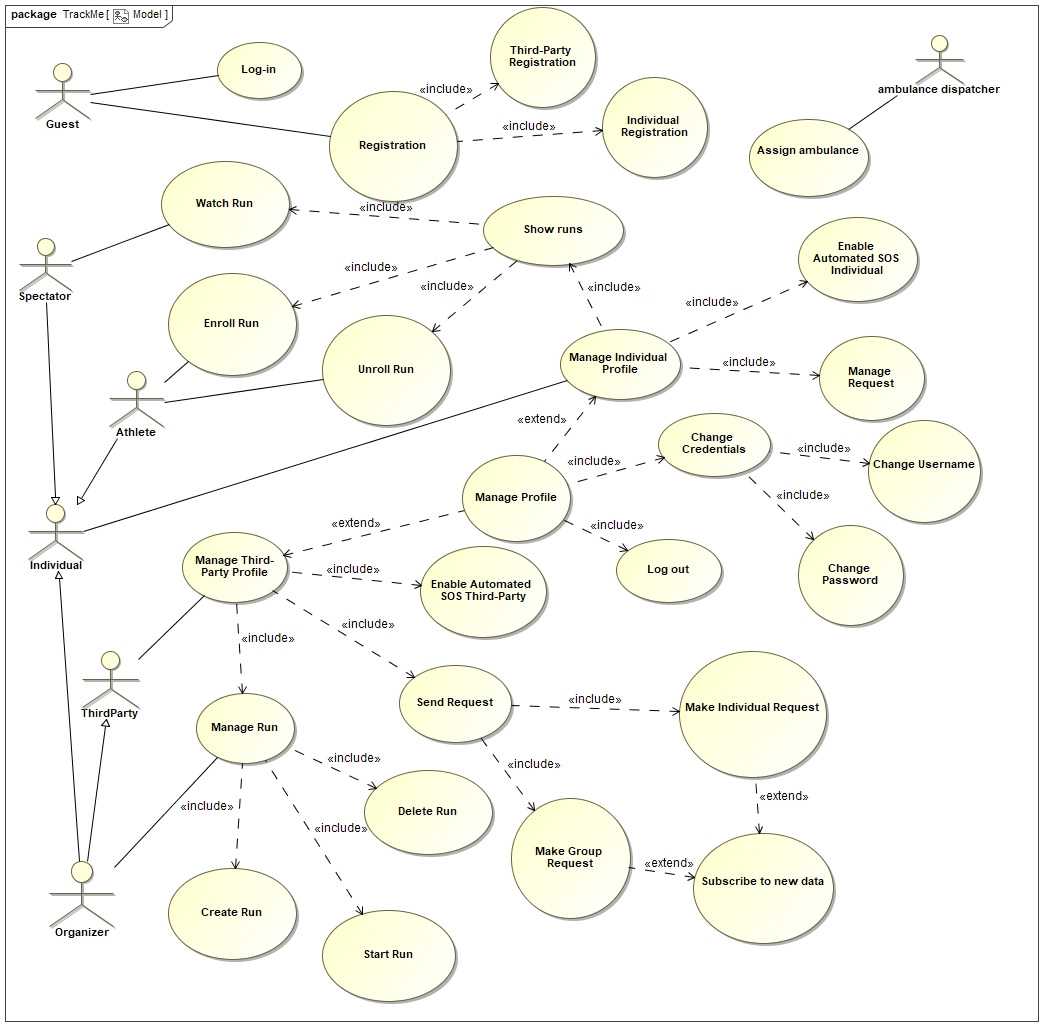
\includegraphics[width=\textwidth,height=160mm]{images/UML/Model.jpg}
        \end{figure}
        \newpage
        \subsubsection{Registration}
        \textit{TrackMe} must provide a registration interface to a guest. 
        
        \begin{usecase}{ Registration}
        \name{Registration}
        \brief{A guest sign up to the application, he can choose to sign on as an individual or as a Third-Party.}
        \actor{Guest.}
        \pre{The guest is on the main page.}
        \bflow{The guest goes on registration page pressing \textit{'Sign-on'} button.}
              {TrackMe asks to the user if he's an Individual or a Third Party. The guest can choose between these two options clicking on the right button}
        \post{The guest can now subscribe as Individual or as a Third-Party}
        \end{usecase}
        
        A  \textit{individual} must provide his/her SSN (Social Security Number) or FC (Fiscal Code) during the registration phase in order to be uniquely identified by \textit{TrackMe} application. In this way, the user is also accepting terms of service and allows \textit{TrackMe} to acquire his/her personal data.
        %use cases table structure
        \begin{usecase}{Individual  Registration}
        \name{Individual Registration}
        \brief{A guest sign up to the application as an Individual.}
        \actor{Guest.}
        \pre{The individual has a valid SSN/FC and he has selected the \textit{Individual} option in the Registration use case.}
        \bflow{The system asks to provide a SSN/FC (based on region) and user personal information such as name, surname, age, gender, e-mail, nationality and optional notes about his health condition.}
              {The individual fills out the requested information and presses the confirm button.}
               {TrackMe asks to provide username and password.}
              {The system registers that user as an Individual and adds it to the  Database.}
        \post{The individual is successfully registered as an Individual.}
        \except{The guest provide a username already present on the database. In this case an error message is printed out the guest must chose a correct username.}
        {If the password chosen is too short an error message is printed out and the guest must chosen an other one.}
      \end{usecase}
        
        
        A \textit{third-party} must provide a VAT number during the registration in order to allow \textit{TrackMe} to check that the submitted VAT is registered and that is issued by an EU Member State.
        
        \begin{usecase}{Third Party User Registration}
        \name{Third Party User Registration}
        \brief{A third party sign up to the application to become an user.}
        \actor{Third Party, TrackMe.}
        \pre{The third party has a valid VAT and it's on the main page.}
        \bflow{The third party goes on registration page pressing \textit{'Sign-on'} button.}
              {TrackMe asks to the user if he's an Individual or a Third Party. The user can choose between these two options.}
              {The third party choose the Third Party option.}
              {TrackMe asks to provide a VAT number and organization personal information.}
              {TrackMe registers the user as a Third Party user and adds it to the Database.}
        \post{The third party is successfully registered as an Third Party User.}
        \end{usecase}
        
        \subsubsection{Log-in}
        The system should provide a login interface to the \textit{User} in order sign into the application.
        
        \begin{usecase}{Individual User Login}
        \name{Individual User Login}
        \brief{An individual sign in to access the application.}
        \actor{Individual, TrackMe.}
        \pre{The individual is already registered and it's on the main page.}
        \bflow{The individual goes on login page pressing \textit{'Sign-in'} button.}
              {TrackMe provides to the \textit{user} a form composed by two text boxes where the user can write and a button to send the form. The first box is the \textit{'username'}, while the latter is the \textit{'password'} field.}
              {The individual writes his username on the \textit{'username'} box and his associated password on \textit{'password'} box and presses the Log-in button.}
              {TrackMe checks username is on the DB and that its associated password is correct.}
              {TrackMe finds that username and its associated password are valid and grants access to the user.}
        \post{The individual is successfully authenticated as \textit{Individual User}.}
        \end{usecase}
        
        \begin{usecase}{Third Party User Login}
        \name{Third Party User Login}
        \brief{A third party sign in to access the application.}
        \actor{Third Party, TrackMe.}
        \pre{The third-party is already registered and it's on the main page.}
        \bflow{The third party goes on login page pressing \textit{'Sign-in'} button.}
        {TrackMe provides to the \textit{user} a form composed by two text boxes where the user can write and a button to send the form. The first box is the \textit{'username'}, while the latter is the \textit{'password'} field.}
        {The third-party writes his username on the \textit{'username'} box and his associated password on \textit{'password'} box and presses the Log-in button.}
        {TrackMe checks username is on the DB and that its associated password is correct.}
        {TrackMe finds that username and its associated password are valid and grants access to the user.}
        \post{The third party is successfully authenticated as \textit{Third-Party User}.}
        \end{usecase}
        
        \subsubsection{Data4Help Request}
        The application may provide an interface that allows \textit{Third-Parties} to send requests to view the data of a specific \textit{individual} or a group of \textit{individuals}. A single individual may accept or refuse this request.
        
        \begin{usecase}{Individual Data Request}
        \name{Third Party Individual Data Request}
        \brief{A third party sends a request to an individual to view his data.}
        \actor{Third Party, Individual, TrackMe.}
        \pre{The third-party is logged-in, it's on the main page and has a valid SSN/FC of a registered individual.}
        \bflow{The third party presses the \textit{'Data-Request'} button.}
              {TrackMe asks if user wants to request data to a specific individual or to get anonymous data of a group of individuals.}
              {The third party presses the button \textit{'Individual'} }
              {TrackMe provides a box called \textit{'SSN/FC'} where the user can write.}
              {The third party writes the individual \textit{'SSN/FC'} and presses the \textit{'Submit'} button.}
              {TrackMe sends the data request to the individual.}
              {TrackMe informs the Third-Party user that the operation succeed.}
        \post{The third party has successfully sent a data request to the individual.}
        \end{usecase}
        
        \begin{usecase}{Third Party Group Data View}
        \name{Third Party Group Data View}
        \brief{A third party views data of a group of individuals.}
        \actor{Third Party, Individual, TrackMe.}
        \pre{The third-party is logged-in and it's on the main page.}
        \bflow{The third party presses the \textit{'Data-Request'} button. Third party is now on the Data-Request page.}
              {TrackMe asks if user wants to request data to a specific individual or to get anonymous data of a group of individuals.}
              {The third party presses the button \textit{'Group'}. Third party is now on the Group subsection of Data-Request page.}
              {TrackMe provides an interface in which a third-party can insert search criteria for group requests.}
        {Third party fills out the form and then presses the button \textit'Send Request'.}
        {TrackMe checks if the number of individuals of the group who matches the search criteria defined on point \textit{a)} is greater than 1000.}
        {TrackMe informs the Third-Party that the operation succeed.}
        \post{The third party has access to the data of a specific group of individuals.}
        \end{usecase}
        
        \begin{usecase}{Third Party Subscribes to New Data}
        \name{Third Party Subscribes to New Data}
        \brief{A third party subscribes to the data of a certain group of individuals.}
        \actor{Third Party,  Individual, TrackMe.}
        \pre{The third-party is logged-in and it's on the Group subsection of Data-Request page.}
        \bflow{TrackMe provides a check-box to allow a third-party to choose if she wants to be subscribed to new data.}
            {Third party checks the \textit{'Subscribe'} box.}
            {TrackMe checks if the request is a valid request.}
        \post{The third party is subscribed to the individuals' data and will receive new data as soon as they are produced.}
        \end{usecase}
        
        \begin{usecase}{Individual Accepts Data Request}
        \name{Individual Accepts Data Request}
        \brief{An individual accepts the request to view his personal data.}
        \actor{Third Party, Individual, TrackMe.}
        \pre{The individual is logged-in and it's on the main page.}
        \bflow{TrackMe sends to the individual a request to view his data. The individual can see that the request was sent by a specific third-party. TrackMe provides two buttons called \textit{Accept} and \textit{Refuse}.}
              {The individual presses the accept button.}
              {TrackMe sends to the third-party a confirmation about his request for that Individual.}
        \post{The third party has access to the Individual data.}
        \end{usecase}
        
        \subsubsection{Connection of External Devices}
        The application may provide an interface that allows \textit{individual} to connect an external device such as smart-watch via Bluetooth or NFC.
        
        Moreover, in case such interface is present, \textit{TrackMe} should be able to interact also with the external device and to acquire data from it.
        
        
        \subsubsection{Automated-SOS enabling}
        
        \begin{usecase}{Third Party Enables Automated-SOS}
        \name{Third-Party Enables Automated-SOS}
        \brief{A Third-Party wants to enable Automated-SOS, a service that guarantees that an ambulance will be called in 5 seconds if an individual's health parameters are below certain thresholds. That individual must be subscribed to the Third Party.}
        \actor{Third party, Automated-SOS}
        \pre{The Third-Party is logged-in, it's on the main page and has not enabled Automated-SOS.}
        \bflow{The Third-Party presses the \textit{'Enable Automated-SOS'} button.}
              {Automated-SOS checks if the user has already enabled the service.}
              {Automated-SOS asks if the user wants to enable Automated-SOS. It provides two buttons called \textit{'Confirm'} and \textit{'Back'}.}
              {Third Party presses the \textit{'Confirm'} button.}
              \post{Third-Party has enabled Automated-SOS and individuals that enabled Automated-SOS can see the third-party in the Automated-SOS third-party list.}
        \end{usecase}
        
        \begin{usecase}{Individual Enables Automated-SOS}
        \name{Individual enables Automated-SOS}
        \brief{An Individual wants to be monitored by a Third-Party: in case his health parameters are below certain thresholds an ambulance will be called within 5 seconds.}
        \actor{Individual, Automated-SOS}
        \pre{The Individual is logged-in, it's on the main page and has not enabled Automated-SOS.
            There is at least one Third-Party that has enabled the Automated-SOS service.}
        \bflow{The Individual presses the \textit{'Enable Automated-SOS'} button.}
              {Automated-SOS checks if the user has already enabled the service.}
              {Automated-SOS asks if the user wants to enable Automated-SOS. It provides a list of Third parties that enabled Automated-SOS. User can choose only one third-party. Automated-SOS also provides two buttons called \textit{'Confirm'} and \textit{'Back'}. The \textit{'Confirm'} button can be pressed only if at least one third-party is selected.}
              {Individual selects a third-party and presses the \textit{'Confirm'} button.}
        \post{Third-Party has enabled Automated-SOS and individuals that enabled Automated-SOS can see the third-party in the Automated-SOS third-party list.}
        \end{usecase}
        
        
        \subsubsection{Automated-SOS Data Management}

        \begin{usecase}{Automated-SOS Data Management}
        \name{Automated-SOS Data Management}
        \brief{The system will periodically check individual's data, and if the thresholds have been overcome, it will automatically notify an ambulance within 5 seconds.}
        \actor{Automated-SOS, Ambulance, Individual, Third Party.}
        \pre{At least one ambulance must be available; the Third Party must have enabled Automated-SOS. The individual has to be subscribed to the Third-Party.}
        \bflow{The system checks the Individual's health parameters and finds that he has overcame the thresholds.}
              {Automated-SOS checks in the ambulance database the nearest one available.}
              {Automated-SOS sends to the selected ambulance a request with the GPS position of the subject in danger.}
              {The ambulance selected should accept the request, otherwise Automated-SOS will notify the second ambulance available and so on until the request is accepted.}
        \post{} % what is the post-condition? There IS a post-condition?
        \end{usecase}
        
        \subsubsection{Run Management}
        
        \begin{usecase}{Third Party Creates a New Run}
        \name{Third Party Creates a New Run}
        \brief{A third party become an \textit{Organizer} and creates a new \textit{run}, where \textit{Athletes} can enroll and \textit{Spectators} can watch.}
        \actor{Third Party, Track4Run.}
        \pre{The Third party is logged-in and it's on the main page.}
        \bflow{The Third party presses a button called \textit{'Track4Run'}. third-party is now on the Track4Run page.}
              {Track4Run provides two buttons: one called \textit{'Create Run'} and one called \textit{'Run list'}.}
              {The third party presses the \textit{'Create Run'} button.}
              {Track4Run asks the user if he wants to create a new run. Track4Run provides a set of boxes called \textit{'Name'}, \textit{'Country'}, \textit{'Date'} ............. and two buttons called \textit{'Confirm'} and \textit{'Back'}.}
              {Third party fills the boxes and then presses the \textit('Confirm') button.}
              {Track4Run asks the user to defines a \textit(path) using ......................................}
              {The Third-Party defines the \textit(path) using ................................... and presses the }
              {Track4Run now recognize the Third Party as an Organizer and add the \textit{run} information to the Run DB.}
              {Track4Run informs the Organizer that the operation succeed.}
        \post{The run is created and its state is \textit{created}. The Third Party becomes an Organizer.}
        \end{usecase}
        
        \begin{usecase}{Organizer Starts a Run}
        \name{Organizer Starts a Run}
        \brief{An Organizer starts a run that he has previously created.}
        \actor{Organizer, Track4Run.}
        \pre{The Organizer is logged-in and it's on Track4Run page. The Organizer must have created at least one run and this run state must be \textit{'created'}.}
        \bflow{The Third party presses a button called \textit{'Run list'}.}
              {Track4Run provides a list of runs that the Organizer has created. The Organizer can select a run from the list. Track4Run also provides a set of buttons when a run is selected. If the run selected state is \textit{created} then there are two buttons called \textit{'Start run'} and \textit{'Delete run'}. If the run selected state is \textit{started} then there is a button called \textit{'Close run'}.}
              {Organizer select a \textit{created} run and presses the \textit{'Start run'} button.}
        \post{The selected run state is now \textit{started} and now Athletes can no longer subscribe to that run.}
        \end{usecase}
        
        \begin{usecase}{Organizer Closes a Run}
        \name{Organizer Closes a Run}
        \brief{An Organizer closes a run that he has previously started.}
        \actor{Organizer, Track4Run.}
        \pre{The Organizer is logged-in and it's on Track4Run page. The Organizer must have created at least one run and this run state must be \textit{'started'}.}
        \bflow{The Third party presses a button called \textit{'Run list'}.}
              {Track4Run provides a list of runs that the Organizer has created. The Organizer can select a run from the list. Track4Run also provides a set of buttons when a run is selected. If the run selected state is \textit{created} then there are two buttons called \textit{'Start run'} and \textit{'Delete run'}. If the run selected state is \textit{started} then there is a button called \textit{'Close run'}.}
              {Organizer select a \textit{started} run and presses the \textit{'Close run'} button.}
        \post{The selected run state is now \textit{closed} and now Spectators can no longer view the Athletes' position of that run.}
        \end{usecase}
        
        \begin{usecase}{Organizer Deletes a Run}
        \name{Organizer Deletes a Run}
        \brief{An Organizer deletes a run that he has previously created.}
        \actor{Organizer, Track4Run.}
        \pre{The Organizer is logged-in and it's on Track4Run page. The Organizer must have created at least one run and this run state must be \textit{'created'}.}
        \bflow{The Third party presses a button called \textit{'Run list'}.}
              {Track4Run provides a list of runs that the Organizer has created. The Organizer can select a run from the list. Track4Run also provides a set of buttons when a run is selected. If the run selected state is \textit{created} then there are two buttons called \textit{'Start run'} and \textit{'Delete run'}. If the run selected state is \textit{started} then there is a button called \textit{'Close run'}.}
              {Organizer select a \textit{created} run and presses the \textit{'Delete run'} button.}
        \post{Any Athlete that was subscribed to that run is no longer subscribed. Athletes can no longer subscribe to that run. That run is deleted from the list of available runs.}
        \end{usecase}
        
        \subsubsection{Run Enrollment}
        
        \begin{usecase}{Individual Enrolls a Run}
        \name{Individual Enrolls a Run}
        \brief{An individual enrolls to a run created by an Organizer.}
        \actor{Individual, Track4Run.}
        \pre{The individual is logged-in and it's on the main page, there is at least a run available that has state \textit{created}.}
        \bflow{The Individual presses a button called \textit{'Track4Run'}.}
              {Track4Run asks the user if he wants to join or spectate a run. Track4Run provides two buttons, one called \textit{'Enroll'} and the other \textit{'Spectate'}.}
              {Individual presses the \textit{'Enroll'} button.}
              {Track4Run provides a list of runs that the user can select. These runs must have the state \textit{created}. Track4Run also provides two buttons: a \textit{'Confirm'} button that can be pressed if and only if at least one run is selected; a \textit{'Back'} button.}
              {Individual selects one run from the list and presses the \textit{'Confirm'} button.}
              {Track4Run now recognize the Individual as an Athlete.}
              {Track4Run informs the Athlete that the operation succeed.}
        \post{The Athlete successfully enrolls the run and his position will be sent to all \textit{Spectators} that spectate that run.}
        \end{usecase}
        
        \subsubsection{Run Watching}
        
        \begin{usecase}{Individual Spectates a Run}
        \name{Individual Spectates a Run}
        \brief{An individual wants to spectate a \textit{run} to view the position of all Athletes participating that run.}
        \actor{Individual, Track4Run.}
        \pre{The individual is logged-in and it's on the main page. There is at least one \textit{started} run.}
        \bflow{The Individual presses a button called \textit{'Track4Run'}.}
              {Track4Run asks the user if he wants to join or spectate a run. Track4Run provides two buttons, one called \textit{'Enroll'} and the other \textit{'Spectate'}.}
              {Individual presses the \textit{'Spectate'} button.}
              {Track4Run provides a list of runs that the user can select. These runs must have the state \textit{started}. Track4Run also provides two buttons: a \textit{'Confirm'} button that can be pressed if and only if at least one run is selected; a \textit{'Back'} button.}
              {Individual selects one run from the list and presses the \textit{'Confirm'} button.}
              {Track4Run now recognize the Individual as a Spectator.}
        \post{The Spectator successfully spectates the run and he has granted access to the position of all Athletes enrolling the selected run until the run state is \textit{closed}.}
        \end{usecase}
    
    \subsection{Design Constraints}
    
        \subsubsection{Standards Compliance}
        
        \subsubsection{Hardware Limitations}
        
        \subsubsection{Other Constraints}
    
    \subsection{Software System Attributes}
        
        \subsubsection{Reliability}
        
        \subsubsection{Availability}
        
        \subsubsection{Security}
        
        \subsubsection{Maintainability}
        
        \subsubsection{Portability}
        
%%%%%%%%%%%%%%%%%%%%%%%%%%%%%%%%%%%%%%%%%%%%%%%%%%%%%%%%%%%%%%
\newpage
\section{Formal Analysis using Alloy}
\renewcommand*{\lstlistlistingname}{Alloy model samples}
\lstlistoflistings
\newpage
%definition of alloy language for Latex
\lstdefinelanguage{Alloy}{
	morekeywords={
		module, open, as,
		private, abstract, sig, extends, in,
		lone, some, one, disj,
		fact, pred, fun, assert,
		run, check,
		for, but, exactly,
		this, not, implies, else, let,
		not, no, set, all, sum,
		iff, or, Int, and,
		none, univ, iden,
	},
	sensitive=true,
	morecomment=[l]{//},
	morecomment=[l]{--},
	morecomment=[s]{/*}{*/},
	morestring=[b]{"},
	literate={->}{${\rightarrow}$}1
	% replacing characters can cause problems when copying from PDF to editor
}[keywords,comments,strings]
\lstset {
    language=Alloy,
    frame=tb,
    breaklines=true,
    tabsize=3,
    showstringspaces=false,
    numbers=none,
    commentstyle=\color{commentgreen},
    keywordstyle=\color{blue},
    stringstyle=\color{red},
    basicstyle=\small\ttfamily, % basic font setting
    escapechar=\&,
    % keyword highlighting
    classoffset=1, % starting new class
    keywordstyle=\color{weborange},
    classoffset=0,
}
\subsection{Data4Help}
    \lstinputlisting[language=Alloy, caption=Data4Help: model definition, firstline=0, lastline=110]{TrackMeAlloyModel.als}
    
    \lstinputlisting[language=Alloy, caption=Data4Help: single individual request, firstline=111, lastline=118]{TrackMeAlloyModel.als}
    \begin{figure}[!htpb]
    	\centering
    	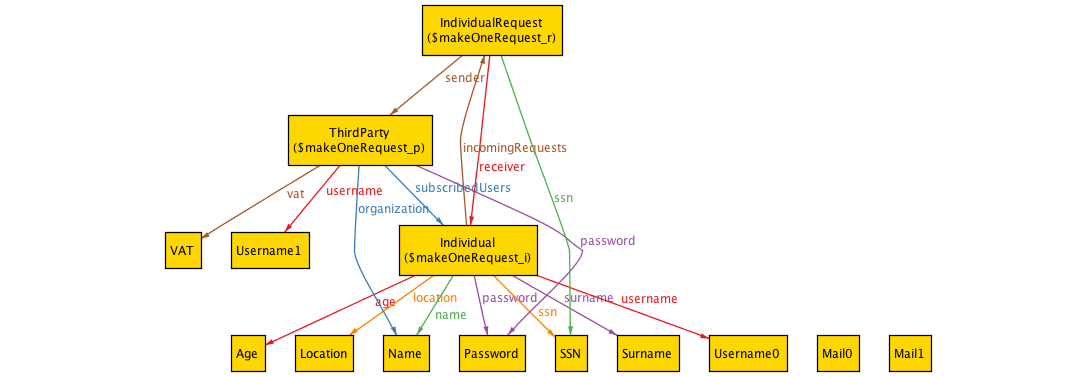
\includegraphics[width=100mm]{images/alloy/makeOneRequest.png}
    \end{figure}
    
    \lstinputlisting[language=Alloy, caption=Data4Help: complete, firstline=119, lastline=125]{TrackMeAlloyModel.als}

\subsection{Automated-SOS}
    \lstinputlisting[language=Alloy, caption=Automated-SOS: model definition, firstline=127, lastline=167]{TrackMeAlloyModel.als}
    
    \lstinputlisting[language=Alloy, caption=Automated-SOS: enable automated-sos, firstline=168, lastline=172]{TrackMeAlloyModel.als}
    \begin{figure}[!htpb]
    	\centering
    	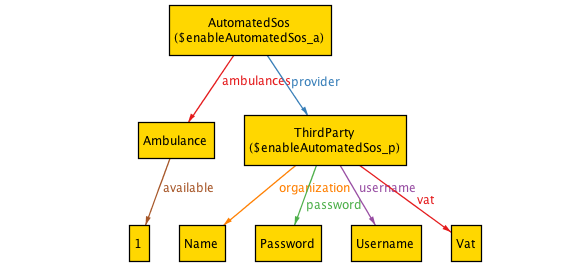
\includegraphics[width=100mm]{images/alloy/enableSos.png}
    \end{figure}
    
    \lstinputlisting[language=Alloy, caption=Automated-SOS: run Automated-SOS, firstline=173, lastline=178]{TrackMeAlloyModel.als}
    \begin{figure}[!h]
    	\centering
    	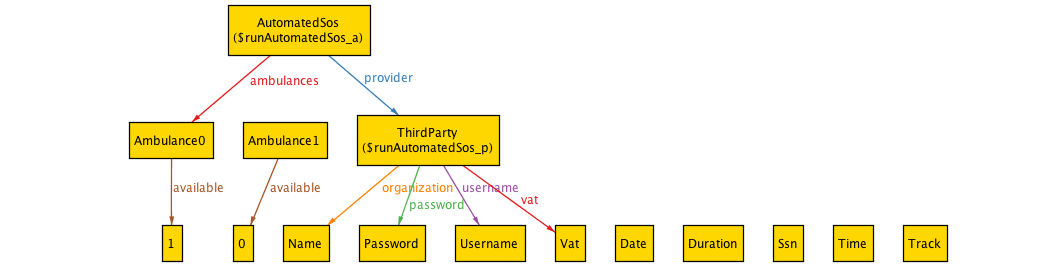
\includegraphics[width=100mm]{images/alloy/runSos.png}
    \end{figure}

\subsection{Track4Run}
    \lstinputlisting[language=Alloy, caption=Track4Run: model definition, firstline=179, lastline=223]{TrackMeAlloyModel.als}
    
    \lstinputlisting[language=Alloy, caption=Track4Run: create a new run, firstline=224, lastline=230]{TrackMeAlloyModel.als}
    \begin{figure}[!htpb]
    	\centering
    	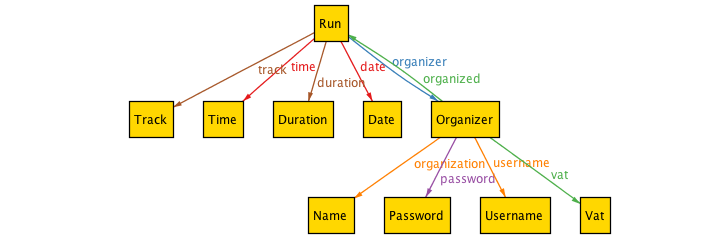
\includegraphics[width=100mm]{images/alloy/createRun.png}
    \end{figure}
    
    \lstinputlisting[language=Alloy, caption=Track4Run: enroll to a run, firstline=232, lastline=239]{TrackMeAlloyModel.als}
    \begin{figure}[!htpb]
    	\centering
    	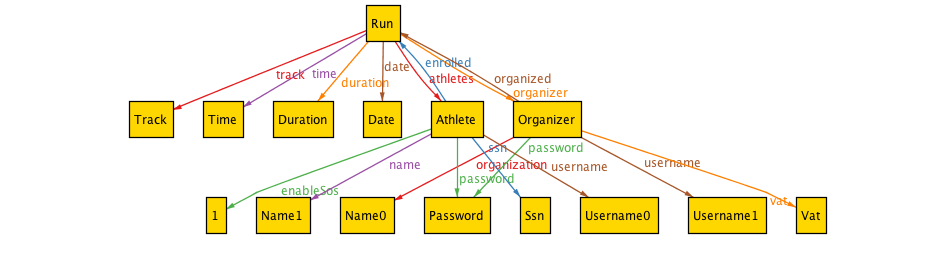
\includegraphics[width=100mm]{images/alloy/enrollRun.png}
    \end{figure}
    
    \lstinputlisting[language=Alloy, caption=Track4Run: watch run, firstline=240, lastline=249]{TrackMeAlloyModel.als}
    \begin{figure}[!htpb]
    	\centering
    	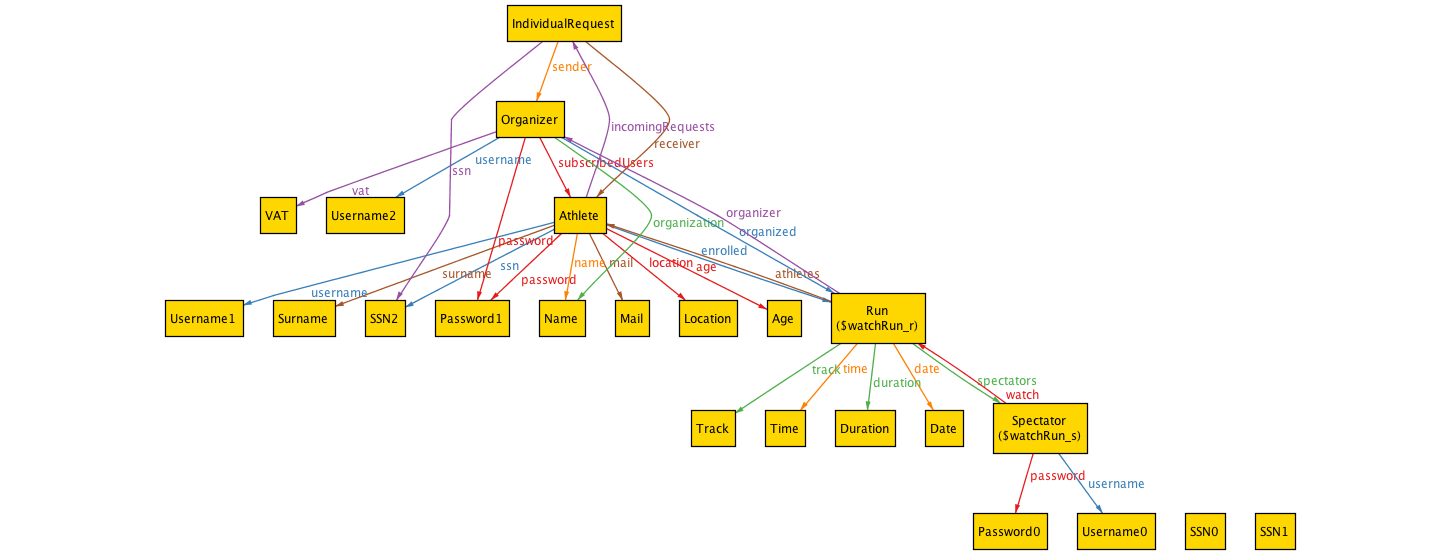
\includegraphics[width=100mm]{images/alloy/watchRun.png}
    \end{figure}
    
    \lstinputlisting[language=Alloy, caption=TrackMe: complete, firstline=250, lastline=259]{TrackMeAlloyModel.als}
    \begin{figure}[!htpb]
    	\centering
    	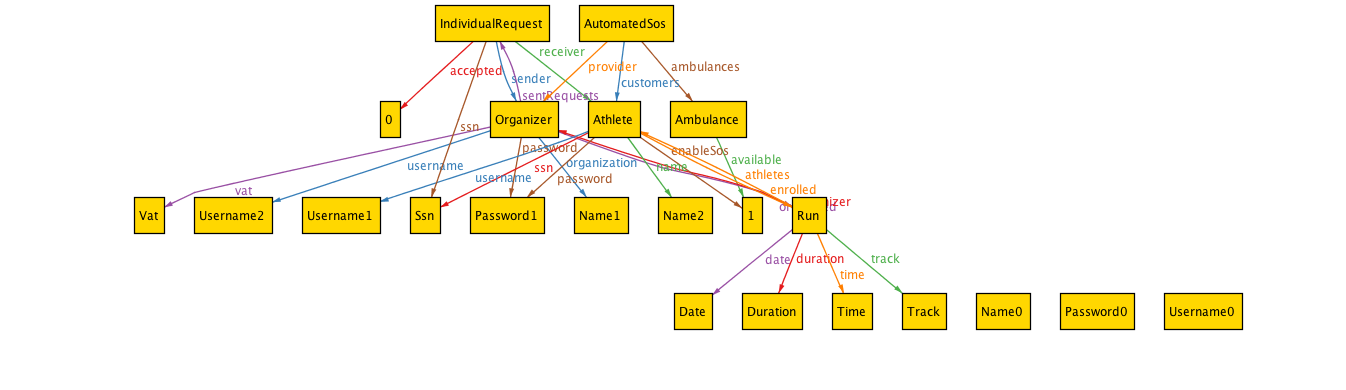
\includegraphics[width=100mm]{images/alloy/trackMe.png}
    \end{figure}
%%%%%%%%%%%%%%%%%%%%%%%%%%%%%%%%%%%%%%%%%%%%%%%%%%%%%%%%%%%%%%
\newpage
\section{Effort Spent}
    \begin{itemize}
        \item[-] \textbf{Davide Rutigliano:}
        
        \item[-] \textbf{Davide Matta:}
        
        \item[-] \textbf{Claudio Ferrante:}
    \end{itemize}

\end{document}
